\section{Internatioanl trade: Standard Assumptions}

What distinguished trade theory from general-equilibrium analysis is the exiatence of a \textbf{hierarchical market structure}.
\begin{itemize}
    \item `International' good markets
    \item `Domestic' factor markets.
\end{itemize}

\begin{question}
    \

    \begin{itemize}
        \item How does the integration of good markets affect good prices?
        \item How do changes in good prices, in turn, affect factor prices, factor allocation, production and welfare?
    \end{itemize}
\end{question}

While these assumptions are less fundamental, we will also often
assume that:
\begin{assumption}
    \

    \begin{itemize}
        \item Consumers have identical homothetic preferences in each country
        (representative agent)
        \item Model is static.
    \end{itemize}    
\end{assumption}

\section{Neoclassical trade}
\textbf{``Neoclassical trade theory''} is characterized by three key assumptions:
\begin{enumerate}
    \item \textbf{Perfect competition} in all markets
    \item \textbf{Constant returns to scale} in production
    \item \textbf{No distortions} 
\end{enumerate}

\begin{note}
    \

    Increasing returns to scale (IRS) are a much more severe issue
addressed by “New” trade theory
\end{note}

Let's first stick to the general case and show how simple revealed preference arguments can be used to establish
two important results:
\begin{enumerate}
    \item \textit{Gains from trade}(Samuelson 1939)
    \item \textit{Law of comparative advantage}(Deardorff 1980)
\end{enumerate}

\subsection{Basic environment}
Consider a world economy with $n=1, 2, \cdots, N$ countries, each populated by $h=1, \cdots, H$ households.

There are $g=1, \cdots, G$ goods:
\begin{itemize}
    \item $y^n \equiv (y_1^n, \cdots, y_G^n) \equiv \text{Output vector in country } n$
    \item $c^{nh}  \equiv (c_1^{nh} , \cdots, c_G^{nh} ) \equiv \text{Consumption vector of household } h \text{ in country } n$
    \item $p^n \equiv (p_1^n, \cdots, p_G^n) \equiv \text{Price vector in country } n$
\end{itemize}

There are $f=1, \cdots, F$ factors:
\begin{itemize}
    \item $v^n \equiv (v_1^n, \cdots, v_F^n) \equiv \text{Factor endowment vector in country } n$
    \item $w^n \equiv (w_1^n, \cdots, w_F^n) \equiv \text{Factor price vector in country } n$
\end{itemize}

\subsubsection{Supply side}
We denote by $\Omega^n$ the set of combinations $(y, v)$ feasible in country $n$,
our assumption of constant returns to scale implies that $\Omega^n$ is a convex set.

\begin{definition}[Revenue function]
    \label{def:revenuefunc}
    \

    The \textbf{revenue function} in country $n$ of a firm producing output $y$ using factors $v$ is a function $r^n(y, v)$ such that:
    \begin{equation}\label{eq:revenuefunc}
        r^n(y,v) \equiv \max_y \{py | (y, v) \in \Omega^n \}
    \end{equation}
\end{definition}

\begin{note}[see Dixit-Norman pp. 31-36 for details]
    \

    \begin{itemize}
        \item Revenue function summarizes all relevant properties of technology;
        \item Under perfect competition, $y^n$ maximizes the value of output in country $n$:
        \[r^n(p^n, v^n) = p^n y^n.\]
    \end{itemize}
\end{note}

\subsubsection{Demand side}
We denote by $u^{nh}$ the utility function of household $h$ in country $n$.

\begin{definition}[Expenditure function]
    \label{def:expendfunc}
    \

    The \textbf{expenditure function} of household $h$ in country $n$ is a function $e^{nh}(p^n, u^{nh})$ such that:
    \begin{equation}\label{eq:expendfunc}
        e^{nh}(p, u) \equiv \min_{c} \{pc | u^{nh}(c) \geq u\}
    \end{equation}
\end{definition}

\begin{note}[see Dixit-Norman pp. 59-64 for details]
    \

    \begin{itemize}
        \item Here factor endowments are in fixed supply, but easy to generalize to
        case where households choose factor supply optimally
        \item Holding $p$ fixed, $e^{nh}(p,u) $ is increasing in $u$.
        \item Household's optimization implies:
        \[e^{nh}(p^n, u^{nh}) = p^n c^{nh} \]
        where $c^{nh}$ and $u^{nh}$ are the consumption and utility level of the household $h$ in country $n$ in equilibrium, respectively.
    \end{itemize}
\end{note}

\subsection{Gains from Trade}
In the next propositions, when we say ``in a neoclassical trade model'',
we mean in a model where equations (\ref{eq:revenuefunc}) and (\ref{eq:expendfunc}) hold in any
equilibrium.
\begin{figure}[ht]
    \centering
    \begin{subfigure}{0.48\textwidth}
        \centering
        \begin{tikzpicture}[scale=1.2]
            % Define the PPF as a quadratic curve
            \draw[thin, domain=0:4, smooth, variable=\x] plot ({\x}, {4-0.25*\x*\x});
            
            % Indifference curve - tangent to PPF at (2,3)
            \draw[thick, blue, dotted, domain=1.6:3.6, smooth, variable=\x] plot ({\x}, {4/\x + 1});
            
            % Autarky equilibrium point
            \filldraw[red] (2,3) circle (2pt) node[anchor=south west] {$y^a = c^a$};
            
            % Autarky price line (tangent to both curves at autarky point)
            \draw[dashed, red] (1,4) -- (4,1) node[pos=0.9, above] {$p^a$};
            
            % Axes
            \draw[->] (0,0) -- (4.5,0) node[right] {$g_1$};
            \draw[->] (0,0) -- (0,4.5) node[above] {$g_2$};
            
            % Labels
            \node at (4.2,0.5) {PPF};
            \node[blue] at (4.3,2.5) {Indifference curve};
        \end{tikzpicture}
        \caption{Autarky Equilibrium}
    \end{subfigure}
    \hfill
    \begin{subfigure}{0.48\textwidth}
        \centering
        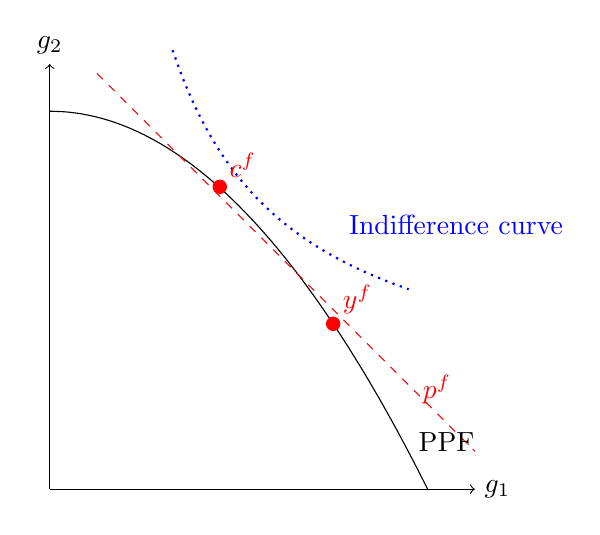
\begin{tikzpicture}[scale=1.2]
            % Define the PPF as a quadratic curve (same as in autarky)
            \draw[thin, domain=0:4, smooth, variable=\x] plot ({\x}, {4-0.25*\x*\x});
            
            % Higher indifference curve for free trade
            \draw[thick, blue, dotted, domain=1.3:3.8, smooth, variable=\x] plot ({\x}, {5/\x + 0.8});
            
            % World price line (different slope than autarky)
            \draw[dashed, red] (0.5,4.4) -- (4.5,0.4) node[pos=0.9, above] {$p^f$};
            
            % Production point (tangent to PPF with world prices)
            \filldraw[red] (3,1.75) circle (2pt) node[anchor=south west] {$y^f$};
            
            % Consumption point (tangent to indifference curve with world prices)
            \filldraw[red] (1.8,3.2) circle (2pt) node[anchor=south west] {$c^f$};
            
            % Axes
            \draw[->] (0,0) -- (4.5,0) node[right] {$g_1$};
            \draw[->] (0,0) -- (0,4.5) node[above] {$g_2$};
            
            % Labels
            \node at (4.2,0.5) {PPF};
            \node[blue] at (4.3,2.8) {Indifference curve};
        \end{tikzpicture}
        \caption{Free Trade Equilibrium}
    \end{subfigure}
    \caption{Equilibria for a Small Country}
    \label{fig:trade_equilibria}
\end{figure}

\subsubsection{Formula of Gains from Trade}
Arkolakis, Costinot, Rodriguez-Clare (AER, 2012)

\begin{assumption}
    \

    \begin{itemize}
        \item CES utility function(Dixit-Stiglitz)
        \[U = \left[\int q(\omega)^{\frac{\sigma -1}{\sigma}}\right]^{\frac{\sigma}{\sigma -1}}\] 
        \item One factor production(labor) and constant RS
        \item `Iceberg' trade costs
        \item Import demand system is CES: artial equilibrium (given wages)
        elasticity of aggregate bilateral trade flow relative to domestic
        demand is $\epsilon $ w.r.t. trade costs $\tau_{ij}$ fo any $i,j$.
    \end{itemize}
\end{assumption}

Define a “foreign shock” as any change in (foreign) endowments and
trade costs that do not affect a country's endowment or its ability to
serve its own market. Define $\hat{W} = \frac{W^{\prime}}{W}$ and $\hat{\lambda}_{jj} = \frac{\lambda_{jj}^{\prime} }{\lambda_{jj}}$

\begin{proposition}
    The change in country $j$'s real income associated with any foreign shock can be computed as $\hat{W}_{j} = \hat{\lambda}_{jj} ^{\frac{1}{\epsilon}}$,
    where $\lambda_{ij} $ is the share of country $j$'s spending on country $i$'s goods.
\end{proposition}

\begin{corollary}
    Gains from TRade relative to autarky can be computed as $\hat{W}_{j} = \lambda_{jj}^{-\frac{1}{\epsilon}} $.
\end{corollary}

\subsubsection{One household per country}
Consider first the case where there is just one household per country, $H=1$.
Without risk of confusion, we drop $h$ and $n$ from all variables.

We denote by:
\begin{itemize}
    \item $(y^a, c^a, p^a)$ the vector of output, consumption and good prices under autarky;
    \item $(y^f, c^f, p^f)$ the vector of output, consumption and good prices under free trade.
    \item $u^a$ and $u^f$ the utility levels under autarky and free trade.
\end{itemize}

\begin{proposition}\label{prop:1}
    \textit{In a neoclassical trade model with one household per country,
    free trade makes all households (weakly) better off.}
\end{proposition}

\begin{proof}
    \

    Under free trade, households can consume at prices $p^f$.
    By definition of the expenditure function, we have:
    \begin{align*}
        e(p^f, u^a) &\leq p^f c^a \\
        &= p^f y^a \\
        & \leq r(p^f, v^f) \\
        &= e(p^f, u^f)
    \end{align*}
    Since $e(p, \cdot)$ is increasing, we get $ u^f \geq u^a$.
\end{proof}

\begin{note}
    \

    \begin{itemize}
        \item Two inequalities in the previous proof correspond to consumption and
        production gains from trade.
        \item Previous inequalities are weak. Equality if kinks in IC or PPF.
        \item Previous proposition only establishes that households always prefer
        ``free trade'' to ``autarky.'' It \textbf{does not} say anything about the
        comparisons of trade equilibria.
    \end{itemize}
\end{note}

\subsubsection{Multiple households per country: domestic lump-sum transfers}
With multiple households per country, moving away from autarky is likely to create winners and losers.
In order to establish the Pareto-superiority of trade, we will need to allow for \textbf{policy instruments}.
We start with \textit{domestic lump-sum transfers} and then \textit{commodity taxes}.

We now reintroduce the index $h$ and denote by:
\begin{itemize}
    \item $c^{ah}$ and $c^{fh}$ the consumption vectors of household $h$ under autarky and free trade;
    \item $v^{ah}$ and $v^{fh}$ the endowment vectors of country $h$ under autarky and free trade;
    \item $u^{ah}$ and $u^{fh}$ the utility levels of household $h$ under autarky and free trade;
    \item $\tau^{h}$ the lump-sum transfer from the government to household $h$ under free trade.
    \footnote{$\tau ^h \leq 0 \Leftrightarrow$ lump-sum tax and $\tau ^h \geq 0 \Leftrightarrow$ lump-sum subsidy.}
\end{itemize}

\begin{proposition}\label{prop:2}
    \

    \textit{In a neoclassical trade model with multiple households per country,
    there exist domestic lump-sum transfers such that free trade is (weakly) Pareto superiority
    than autarky in all countries.}
\end{proposition}

\begin{proof}
    \

    For any $h$, set the lump-sum transfer $\tau^h$ such that:
    \[\tau ^h = (p^f - p^a)c^{ah} - (w^f - w^a)v^{fh}.\]
    Budget constraint unde rautarky implies that: $p^a c^{ah} \leq w^a v^{fh}. $
    Therefore, we have:
    \[p^f c^{ah} \leq w^f v^{fh} + \tau ^h.\]
    Thus $c^{ah} $ is still int he budget set of household $h$ under free trade.
    
    By definition, the government revenue is given by:
    \begin{align*}
        - \sum \tau ^h &= (p^a - p^f) \sum c^{ah} - (w^a - w^f) \sum v^{fh} \\
        &= (p^a - p^f) y^a - (w^a - w^f) v^f \\
        &= -p^f y^a + w^f v^f \\
        & \geq -r(p^f, v^f) + w^f v^f \\
        &= -(p^f y^f - w^f v^f) = 0.
    \end{align*}
\end{proof}

So, each household can buy its autarky consumption bundle at free trade prices and still have some money left.
But, the government must know individual preferences to implement the transfers.

If it does not, households can manipulate mechanism by altering their announcements or
autarky behavior. In other words, lump-sum transfers typically are
not \textcolor{red}{incentive compatible}.

\subsubsection{Multiple households per country: commodity taxes}
We now restrict the set of instruments to commodity taxes/subsidies.

Suppose that the government can affect the porices faced by households under free trade
by setting $\tau ^{good}$ and $\tau ^{factor}$:
\begin{align*}
    p^h &= p^f + \tau ^{good} \\
    w^h &= w^f + \tau ^{factor}.
\end{align*}

\begin{proposition}\label{prop:3}
    \

    \textit{In a neoclassical trade model with multiple households
    per country, there exist commodity taxes/subsidies such that free
    trade is (weakly) Pareto superior to autarky in all countries.}
\end{proposition}

\begin{proof}
    \

    Consider two following taxes:
    \begin{itemize}
        \item $\tau ^{good} = p^a - p^f$
        \item $\tau ^{factor} = w^a - w^f$
    \end{itemize}
    By construction, household is indifferent between autarky and free trade.
    Now consider the government revenue:
    \begin{align*}
        - \sum \tau ^h &= \sum \tau ^{good} c^{ah} - \sum \tau ^{factor} v^{fh} \\ 
        &= (p^a - p^f) \sum c^{ah} - (w^a - w^f) \sum v^{fh} \\
        &= (p^a - p^f) y^a - (w^a - w^f) v^f \\
        &= -p^f y^a + w^f v^f \\
        & \geq -r(p^f, v^f) + w^f v^f \\
        &= -(p^f y^f - w^f v^f) = 0.
    \end{align*}
\end{proof}